% !TEX root = main.tex

本课程采用书目Rafael C. Gonzalez \& Richard E. Woods, \emph{Digital Image Processing (3rd ed)}\footnote{\url{http://www.imageprocessingplace.com}}。

\section{概述}
任何图像本质上就是一个二维函数,x和y是空间坐标,在任何一对空间坐标上的函数值称为该点的强度或灰度。
当x, y和幅值为有限的、离散的数值时,就称这个图像为\textbf{数字图像}。
数字图像处理的输入为图像,输出为图像或图像的子集。

基本步骤:图像获取、图像滤波和增强、图像复原、彩色图像处理、小波与分辨率处理、压缩、形态学处理、分割、表示和描述、目标识别。

\section{数字图像基础}
\subsection{人类视觉}
\begin{itemize}
\item 人的视觉由眼睛中两部分光接收器(感受细胞)组成的:\underline{锥状体}和\underline{杆状体}。
\item 成像原理:与光学透镜相似,但适应性强。看远处物体,肌肉会迫使晶状体变得扁平,晶状体的聚焦中心向前移动;物体离眼睛近时,肌肉使晶状体变厚,光心向视网膜成像区域靠近。
\item 韦伯比:$\Delta I_c/I$,度量人的眼睛特定的\underline{适应级别}对\underline{亮度变化}的辨别力。在\textbf{低的照明}级别,\textbf{亮度辨别较差}(杆状体起作用)。在背景照明增强时,亮度辨别得到明显的改善(锥状体起作用),即对亮的东西敏感。
\item 亮度不是简单的强度函数,下面是两个现象
\begin{itemize}
	\item 视觉系统倾向于不同强度区域边界周围的欠调(undershoot)和过调(overshoot)
	\begin{figure}[H]
	\centering
	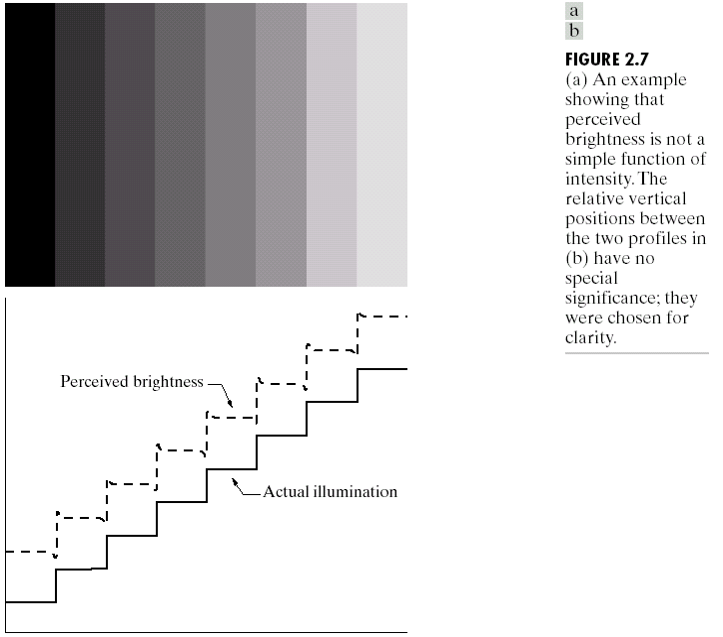
\includegraphics[width=0.5\linewidth]{fig/undershoot-overshoot.png}
	\end{figure}
	\item 同时对比现象
	\begin{figure}[H]
	\centering
	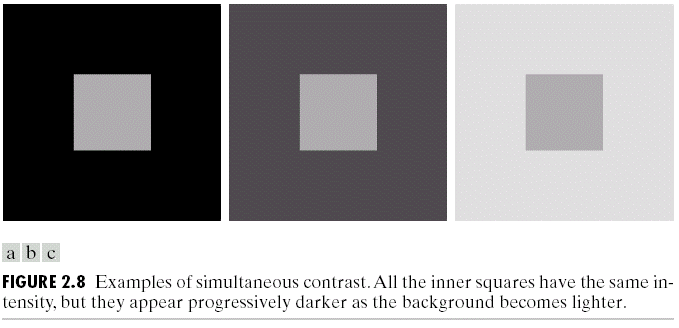
\includegraphics[width=0.5\linewidth]{fig/simultaneous-contrast.png}
	\end{figure}
\end{itemize}
\end{itemize}

\subsection{图像数字化}
图像数字化包括两个步骤
\begin{itemize}
\item 取样(时空域):剖分为像素,用一个像素值代替这一块,$f(x,y)\in[0,+\infty)$
\item 量化(光色强度):变为$[0,255]$之间的整数
\end{itemize}
\[f(x,y)=\bmat{f(0,0) & f(0,1) & \cdots & f(0,N-1)\\f(1,0) & f(1,1) & \cdots & f(m)}\]
即数字图像包括位置属性$(x,y)$和像素大小$f(x,y)$两个特征,用上面的二维矩阵表示,每个元素称为图像的像素。
\begin{itemize}
\item 像素越大越精确,每一块分得越细
\item 计算机中字节处理最快,所以才用8位色(256位)
\end{itemize}

两种不同的分辨率
\begin{itemize}
\item 空间分辨率:\textbf{图像中可分辨的最小细节},即图像大小(行$\times$列)
\item 灰度分辨率:\textbf{一个像素值单位幅度上包含的灰度级数},通常是2的整数幂级数,如:用一个byte存一个像素值为256级
\begin{itemize}
	\item 人眼对灰度分辨率的敏感程度与图像内容复杂程度有关,如更偏爱人脸,而对人群不敏感
	\item 当灰度分辨率不够,会产生伪轮廓
\begin{figure}[H]
\centering
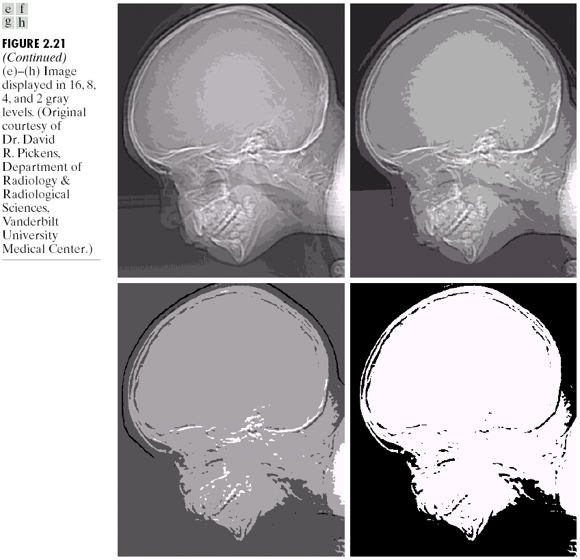
\includegraphics[width=0.5\linewidth]{fig/pseudo-contour.png}
\end{figure}
\end{itemize}
\end{itemize}

放大与缩小:近邻插值、双线性插值

\subsection{像素间基本关系}
\begin{definition}[邻域]
坐标为$(x,y)$的像素$p$的
\begin{itemize}
\item 4邻域$N_4(p)=\{(x-1,y),(x+1,y),(x,y-1),(x,y+1)\}$
\item 对角相邻像素$N_D(p)=\{(x-1,y-1),(x+1,y-1),(x-1,y+1),(x+1,y+1)\}$
\item 8邻域$N_8(p)=N_4(p)\cup N_D(p)$
\end{itemize}
\end{definition}

\begin{definition}[邻接性]
数字图像的邻接需要满足\textbf{灰度值的邻接}和\textbf{物理位置的邻接}。
考虑$V\subset[0,255]$,有三种邻接性:
\begin{itemize}
	\item 4邻接:$q\in N_4(p)$且$q,p\in V$
	\item 8邻接:$q\in N_8(p)$且$q,p\in V$
	\item m邻接混合邻接:要么(1)4邻接,要么(2)$q\in N_D(p)$且$N_4(p)\cap N_4(q)\notin V$
\end{itemize}
若$S_1$中的某些像素和$S_2$中的某些像素邻接,则这两个集合是邻接的。
\end{definition}

注意混合邻接是为了消除8邻接的二义性,见下图。
\begin{figure}[H]
\centering
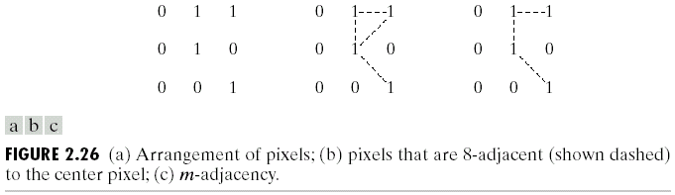
\includegraphics[width=0.6\linewidth]{fig/adjacency.png}
\end{figure}

\begin{definition}[通路]
若$(x,y)$到$(s,t)$有4/8通路,则存在
\[(x_0,y_0),(x_1,y_1),\ldots,(x_n,y_n)\]
其中$(x_0,y_0)=(x,y),(x_n,y_n)=(s,t)$且$(x_i,y_i)$和$(x_{i-1},y_{i-1})$是4/8邻接的
\end{definition}

\begin{definition}[连通集]
如果S中全部像素之间存在一个4/8通路,或者说S仅有一个连通分量,那么称S是4/8连通集。 
\end{definition}

% 2.1、2.6、2.9、2.11、2.15